\chapter{Introduction}
\label{ch:introduction}
Increased competition and complexity of the problems many companies are solving today, constantly change how software is developed. Software development is getting increasingly more focused towards having short and independent release cycles based on individual features rather than entire applications. Solving complex problems often yield a very complex and fragile solution, but the most successful tech companies have succeeded in utilizing a new architecture pattern, namely Microservices. By creating microservices, changing development processes and team structure drastically, modern tech companies create innovative and resilient software quicker than ever before.

Several factors has made this new paradigm for developing big scale distributed applications possible. Cloud computing has made it possible to buy computing resources when needed, cheap and fast. Virtualization and lately containerization makes it possible to create isolated environments, enabling partitioning of applications, into a subset of components that can be developed and deployed independently. Dynamic orchestration of containers makes it possible to ensure correct capacity and redundancy of application components automatically. Segmentation of the applications in turn makes it possible to maintain a acceptable level of complexity of the source code improving maintainability and increasing agility.

\section{Process}
This area of software engineering has seen a major growth in recent years, and has become very information saturated with blog posts, conferences, books, research articles and so on. With the high variety of sources and subjects of interests, it becomes a question of constantly evaluating the credibility and the usability of any pattern, language, tool or framework. This area incorporates a high amount of aspects of software engineering, making it inherently hard to understand to its fullest, if not impossible. 

This thesis has taken outset in finding a partner that could help identify specific challenges, which in turn could be solved using a subset of the available theory, practice and technology in this area, this partner was after careful consideration found to be Danske Bank. Danske Bank in turn introduced a complicated case, the Customer Agreement System (BCA), where resilience was stated as the major concern for the future of the system by involved partners. Several complicated aspects were uncovered, in the definition of the resilience term, creating the need for a better understanding of the evolution of architecture and cloud computing as a term.

\section{Knowledge Sharing}
A rising trend of knowledge sharing has started, where online accessible conference talks and a high quantity of open source projects inspire and help developers solve common challenges. Conferences focus on new open source technology, system architecture, working process and organisational structure, all with a common goal: speeding up software development and the ability to solve increasingly difficult problems. Conferences are either entirely committed to or has tracks about topics like Cloud Computing, Agile Development, Domain Driven Design, Microservices, NoSQL, Docker, Cassandra among many others \cite{george2016it}. Company internal projects that prior was only internal accessible, are increasingly made open source, giving developers very advanced tools to create elegant and efficient solutions quickly. These projects are freely accessible, with well known support challenges where developers can find help with specific challenges utilizing the projects. The Cloud Native Computer Foundation\footnote{\url{https://www.cncf.io/}} (CNCF) is a foundation based entirely on helping non-software focused companies become cloud native: utilizing the power of containerization, and dynamically orchestrated microservices.

The entire movement started when Amazon, an electronic commerce company known for their cloud computing solution, announced Amazon Web Services in 2006. It meant that anyone could register and rent virtual machines for hosting distributed applications. Since then, virtualization has been further revolutionised with the introduction of container technology, which was made open source through the Docker initiative in 2014. Docker made it possible to start up new independent and isolated environments in seconds, something Google, had developed internally because they needed it \cite{bernstein2014containers}. What is somewhat a trademark for the entirety of the cloud native movement, has sprung out of a big variety of needs: serving massive amounts of users, creating reliable applications, the ability to update and add functionality often and easily, minimize integration complexity and technology lock in. In the end the focus should be on solving new problems and not on dealing with an forever growing monolithic application. Microservices have sprung out as a trend in real world use \cite[p.~1]{newman2015microservices}.

\section{Microservices}
Monolithic applications were a result of technological boundaries and made developing good design a major challenge. These boundaries have disappeared, pushing developers towards more thoughtful design of applications. Developers today need to put emphasis on understanding the underlying challenges in the particular domain, identifying the optimal architecture that supports the context \cite[t.~17:00]{evans2016tackling}. High complexity and a strict time to market make problem solving hard. It is therefore very important to optimize the entire process from identification of a correct solution, through development and deployment of the feature. There are three clear factors in this process: technology utilization, correct working process and organisational structure \cite[t.~12:16]{george2016it} \cite[preface]{newman2015microservices}. 

The amount of available languages, frameworks and tools have grown tremendously, making it possible to solve complex problems easier and quicker than before. Utilizing available technology is uttermost important to achieve the best solution for a given problem. Traditionally speaking, organisations often divided people into departments according to their specific competences. Development project would therefore span several departments, creating a need for standardization of tools, languages and working processes. This inherently limits the amount of innovation possible, engineers are forced to solve all problems in a predetermined way, resulting in similar solutions for very diverse problems \cite[t.~14:20]{fowler2014microservicesoamonolith} \cite[00:30]{kniberg2014spotify} \cite{murer2015fifteen} \cite[17:00]{meshenberg2016microservices}. 

The organisation structure's impact on software development has been broadly acknowledged \cite{fowler2014microservices, newman2014demystifying}, and companies are therefore breaking pre-existing organisational structures, prohibiting fast and agile development. Many tech companies have openly talked about their innovative ways of working, that has allowed them to improve the amount of innovation and the productivity of their software engineers \cite[00:30]{kniberg2014spotify} \cite[16:00]{meshenberg2016microservices}. By having a strong focus on having small, strong, cross-functional and self-organising teams that have "end-to-end" responsibility for the features they build. Teams have an overall mission, knowledge of their specific product strategy and short-term goals that help keep the team on the wished path. Each team is given autonomy, responsible for finding the best way for the team to develop new features, which features the team should implement and how they work together. Everyone in the team is located in the same physical location, creating the optimal conditions for good collaboration across skill-sets \cite[01:00]{kniberg2014spotify} \cite{gray2006conversation}.

\begin{figure}[!htb]
  \begin{center} 
	  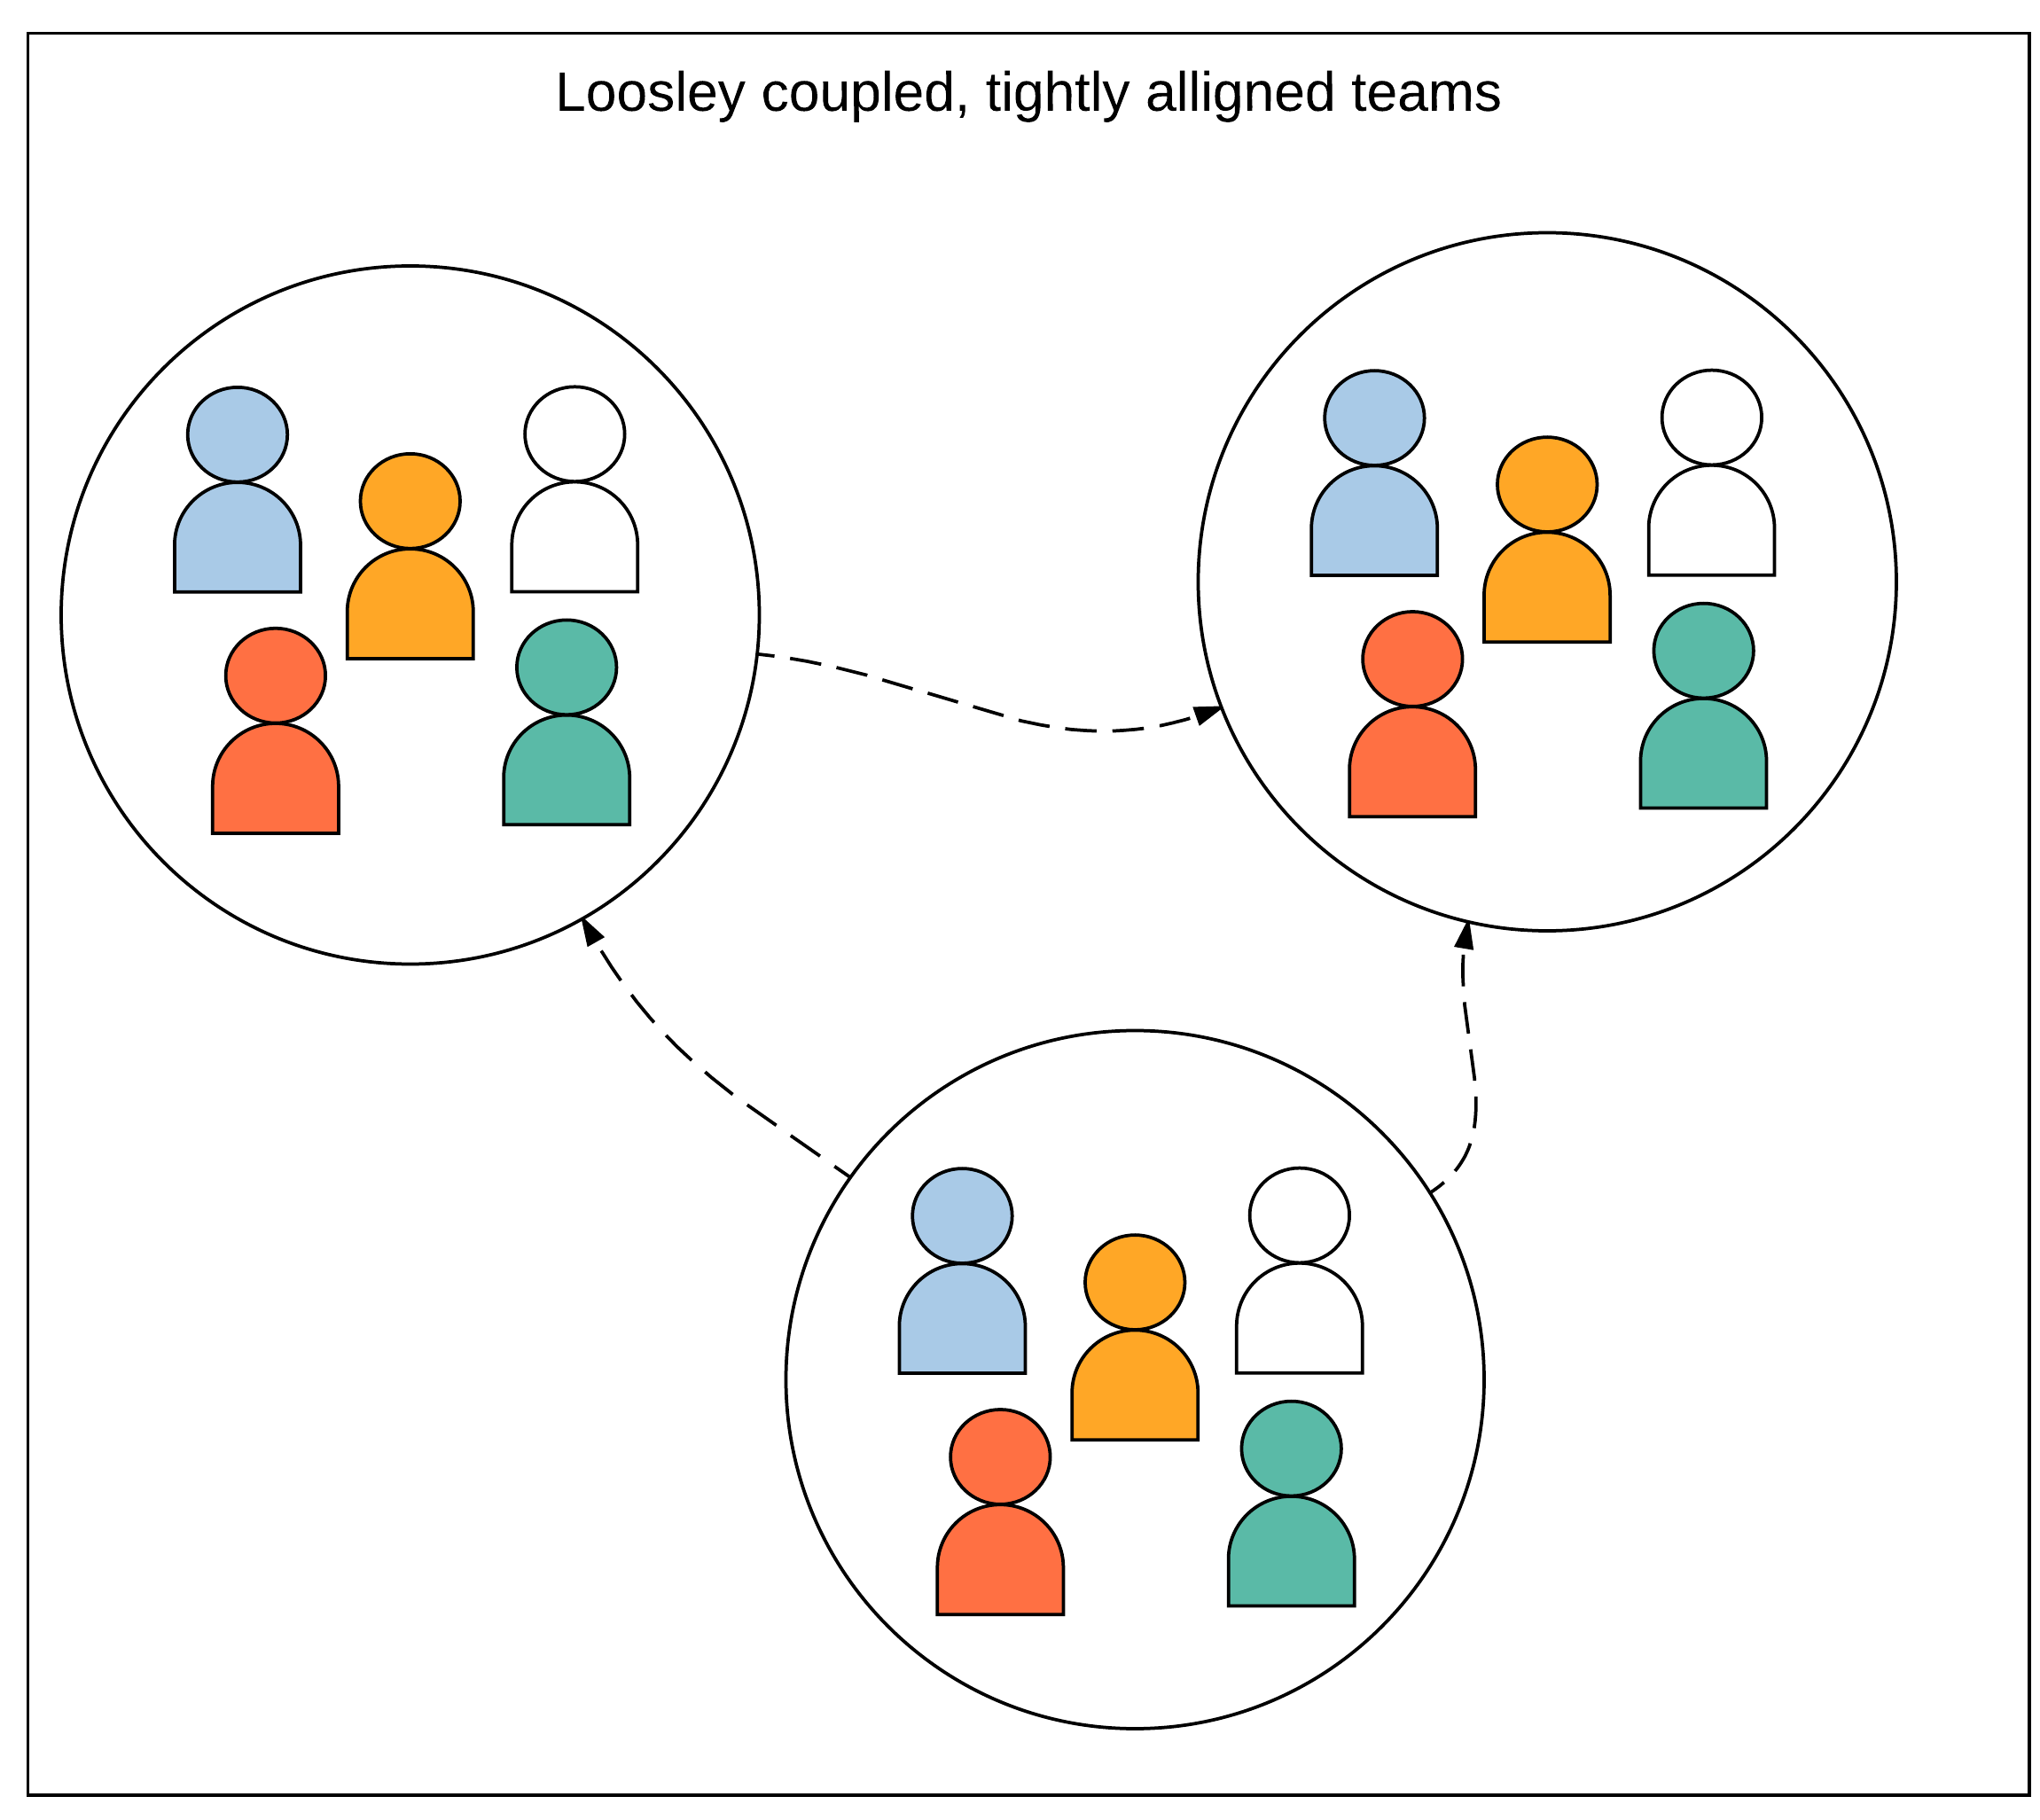
\includegraphics[scale=0.08]{introduction_squads}
  \end{center}
  \caption{Spotify team structure \cite{kniberg2014spotify}}
  \label{fig:introduction_squads}
\end{figure}

This is a completely new way of designing an organisation, which consequently removes pre-existing process and organisation inhibitors. It is possible for each team to create and release features independently, minimizing waiting time between teams. At the same time teams are responsible for what they create, removing handoffs between teams. The focus is loosely coupled but tightly aligned teams.
It is important that organisation and process inhibitors are removed before utilizing microservices as an architecture choice \cite{meshenberg2016microservices}. This will make it possible to utilize available technology to the fullest, by allowing teams to choose which technology is used for the development of the separate features \cite{fowler2014polyglot}. 


\section{Resilience}
The internet, and the services it makes available, has in recent years has grown exponentially \cite[p.~4]{nygard2007release}, the services are essential for users, making consequences of down time increasingly severe. Consequences of downtime are hard to estimate but can effect user satisfaction and trust, and loss of brand and reputation incurring direct and indirect bottom line losses \cite[p.~26]{beyer2016siteReliabilityEngineering}. It is generally acknowledged that services available on the internet are not suficiently resilient \cite{sterbenz2010resilience}. Designing systems with an increased scale and reach incurs a need for optimizing architecture so that it mitigates failure \cite[p.~4]{nygard2007release}, focus needs to be shifted to incorporate the entire lifetime of the application, not only focusing on the development process:

\tquote{Software engineering has this in common with having children: the labor before the birth is painful and difficult, but the labor after the birth is where you actually spend most of your effort. Yet software engineering as a discipline spends much more time talking about the first period as opposed to the second, despite estimates that 40–90\% of the total costs of a system are incurred after birth}{Beyer et al.}{2016}

Due to rapid growth in scale and complexity, it is increasingly important to acknowledge that failure is bound to happen, and reducing the risk of failures and the its effects essential \cite{abid2014toward} \cite[p. 117]{nygard2007release} \cite{tseitlin2013antifragile} \cite{krishnan2012weathering}. Gone are the days where developers only focused on development and deployment, and maintenance of a system was distant processes in the hands of the operations team. The microservice community embraces ownership "You build it, you run it" \cite{gray2006conversation} is the new mantra, embracing deployment and maintenance and focusing on how to make system more resilient when in production \cite[p.~6]{nygard2007release}. Consequently the stability patterns and their antipatterns have to be analysed (how is failure avoided and what enhances failure).

Gaining insights into the microservice and cloud native communities is not easy, it can be very time consuming to understand which problems a given architectural pattern or open source technology can help solve. There are several unclear parts of this area, many different parties are informing about failure and resilience, but no clear definition of the terms exist. In turn different parties emphasize different aspects and solutions to resilience, without a clear indication of which resilience aspect the specific architecture, language, framework or tool serves as a solution to. There is a clear gap between the available resources and a concrete definition of which aspect of resilience, if any, it solves. It requires intricate knowledge of the infinite amount of available languages, frameworks and tools to evaluate which to use in a given situation and how to quantify the given results of utilizing one.

\section{Problem formulation}
\label{sc:problem_formulation}

\begin{itemize}  
\item 1.a How can cloud computing be used to solve availability, performance and maintainability requirements for enterprise applications?
\item 1.b How can cloud computing be used in an enterprise application architecture?

\item 2.a How are enterprise application challenges and possible solutions affected by the application domain?
\item 2.b How does the enterprise application domain affect challenges and possible solutions?
\item 2.c How does the domain shape the challenges in a specific application architecture?
\item 2.d How does the domain and organization shape the challenges in a specific application architecture?

\item 3.a How does a distributed application architecture deal with a single point of failure?
\item 3.b How is single point of failure avoided in a distributed application architecture?

\item 3.c How is the optimal application architecture and distribution method determined and evaluated?
\item 3.d How is the enterprise application architecture determined?
\item 3.e How is the enterprise application architecture evaluated?
\end{itemize}

\subsection*{Notes}
How are the challenges and their optimal solution affected by the specific application?

What determines the optimal application architecture, database and distribution?

How is the optimal application architecture, database and distribution determined?

System architecture:
How is application data optimally stored?
How is application data optimally distributed?

How are application updates optimally executed?
How are updates 

How is the system distributed

This area has been named cloud computing, 

Big cloud computing platforms are now available, offering server rental with 

From these requirements big cloud platforms have been started, 

These requirements has started big scale initiatives in cloud computing, has generated new tools and databases available for development of distributed big scale enterprise applications. 

Creating a need for developers to explore and evaluate which of the many platforms to choose, 

\section{The Solution}
The microservice architecture was investigated due to its focus on designing battle tested and resilient systems. By increasing the granularity of system subdivision, a higher regard to detail is attainable, making it possible to release often and fast, identify and solve problems quickly and correctly and create systems with a manageable complexity. The microservice architecture improves service availability by dictating small and independent services, with focus on individual features instead of entire products, decentralizing data management, automating infrastructure management and design services for resilience. Cloud Computing was in turn investigated as technology it makes replication possible by isolating services into separate environments, making it possible to improve capacity, introducing redundancy and thereby removing single point of failure. 

Resilience consists of dependability and adaptivity. Dependability makes it possible to quantify system resilience, by introducing availability and robustness as quality measures. Adaptivity consists of four different measures: Robustness, Fault Tolerance and Avoidance, Recovery time and Capacity and redundancy. Adaptivity and dependability correlates, improving either of the four subcomponents of adaptivity increases the dependability, and therefore resilience of a system. A test was designed and conducted to show the effects of capacity and redundancy on availability. The amount of load was varied on three differently scaled systems, showing that increasing capacity, increased the amount of throughput the system could withstand, while fulfilling high availability requirements. The maximum throughput was not increased linearly with the increase of capacity, meaning that processing power was not exhausted on individual nodes in cluster configurations with 5 and 10 nodes. This was contributed to limitations in the load balancer of Kubernetes being incapable of distributing the load on all replicas at very high throughputs. 